\chapter[Planejamento da Primeira Iteração]{Planejamento da Primeira Iteração}

A seguir pode-se verificar as histórias de usuárias organizadas com suas respectivas features e épicos. Cada história de usuário apresenta:

\begin{itemize}
	\item Título;
	\item Valor de négocio, sendo classificado em 5 nivéis: Deve ter, ótimo, bom, médio e bom ter, seu nível de importância é respectiva a ordem de apresentação, ou seja, deve ter (mais importante) e bom ter (menos importante);
	\item Quem: Indicando o agente;
	\item O que: Indicando o que faz;
	\item Porque: Indicando o objetivo;
	\item Critérios de Aceitação: Indicando formas de usar a funcionalidade implementada em uma história;
	\item Pontos: Indicando o grau de dificuldade de implementação da história.
\end{itemize}

\begin{enumerate}
	\item \textbf{Épico:} Gerenciamento de Demanda
		\begin{enumerate}
			\item \textbf{Feature:} Manutenção de Demanda
				\begin{enumerate}
					\item \textbf{História 01}
						\begin{figure}[H]
						    \centering
							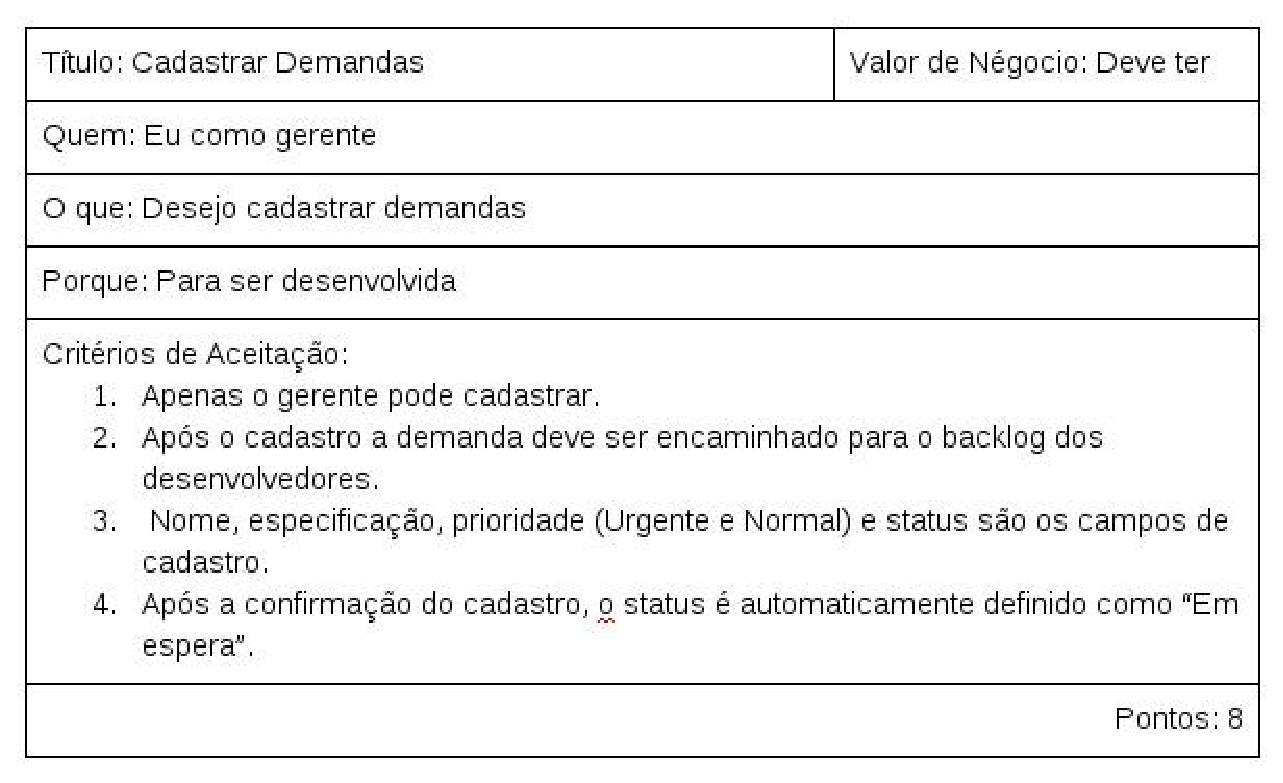
\includegraphics[keepaspectratio=true,scale=0.8]{figuras/iteracao_1/historia_1.eps}
						    \caption{Iteração 1 - História de Usuário}
						    \label{fig:historia1}
						\end{figure}
						
					\item \textbf{História 02}
						\begin{figure}[H]
						    \centering
							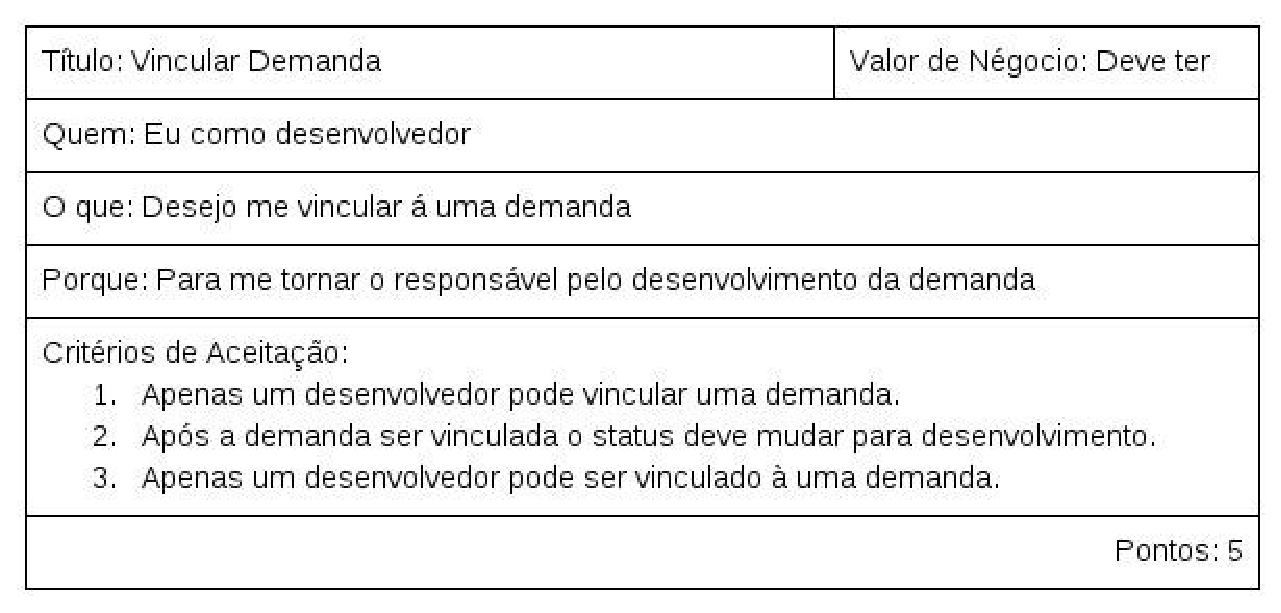
\includegraphics[keepaspectratio=true,scale=0.8]{figuras/iteracao_1/historia_2.eps}
						    \caption{Iteração 1 - História de Usuário}
						    \label{fig:historia1}
						\end{figure}

					\item \textbf{História 03}
						\begin{figure}[H]
						    \centering
							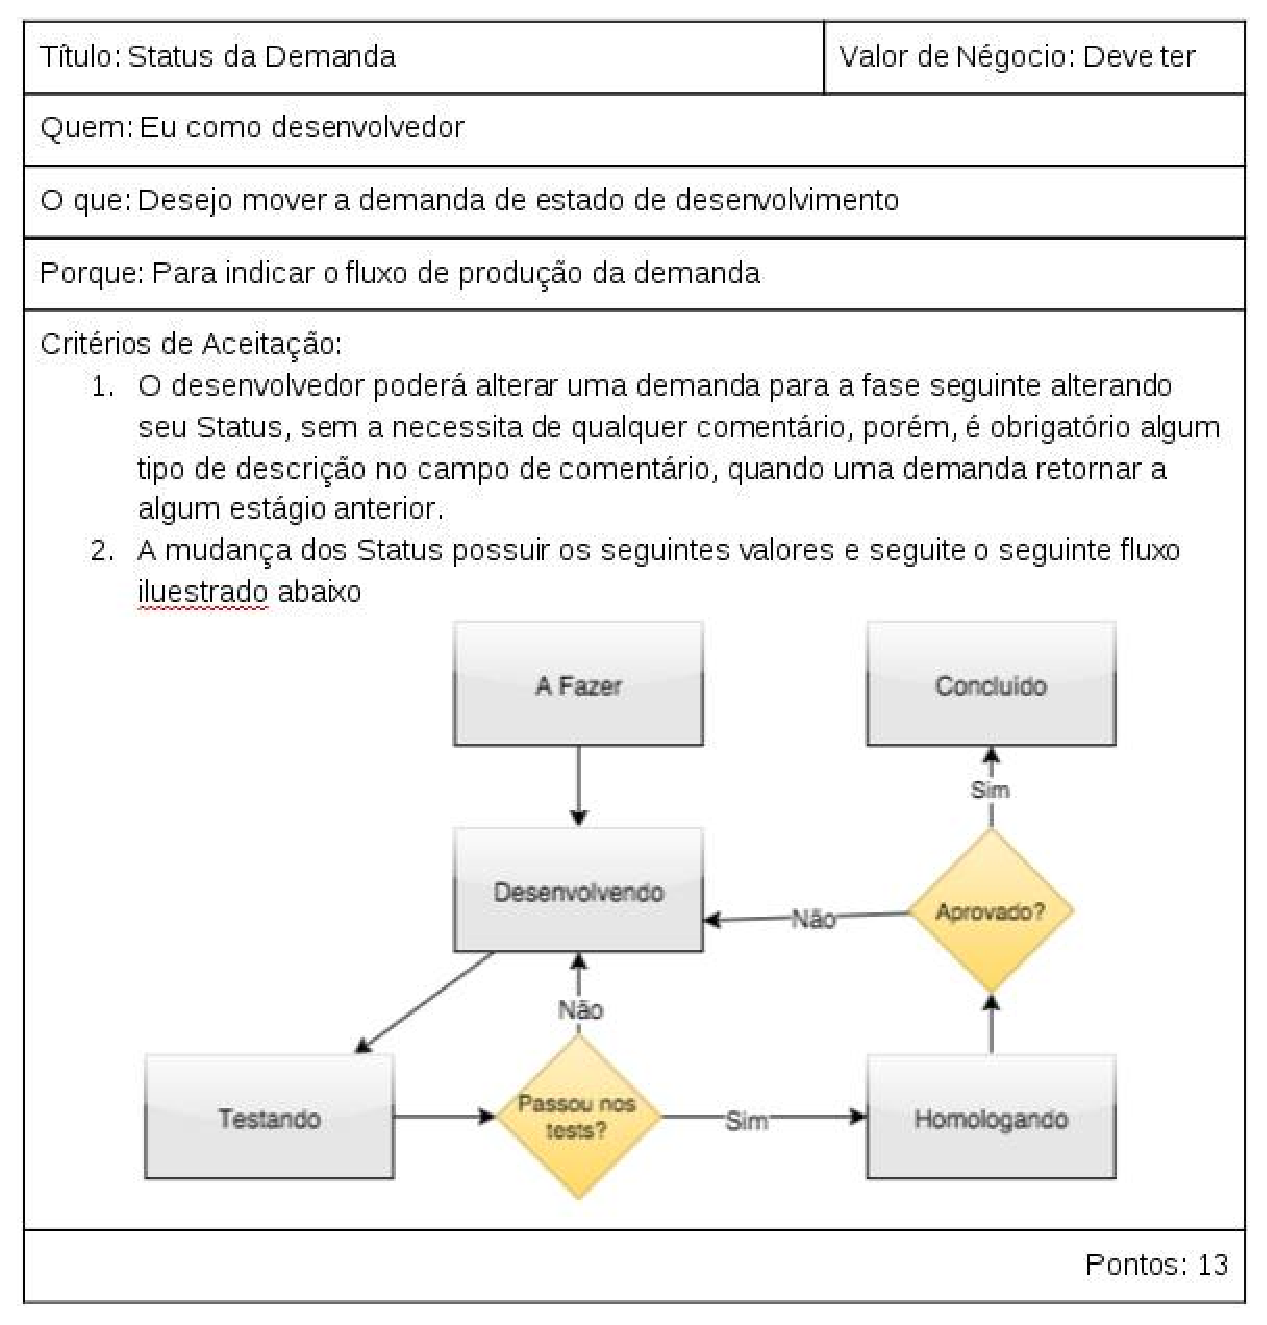
\includegraphics[keepaspectratio=true,scale=0.8]{figuras/iteracao_1/historia_3.eps}
						    \caption{Iteração 1 - História de Usuário}
						    \label{fig:historia1}
						\end{figure}
				\end{enumerate}

			\item \textbf{Feature:} Acompanhamento de Demanda
				\begin{enumerate}
					\item \textbf{História 04}
						\begin{figure}[H]
						    \centering
							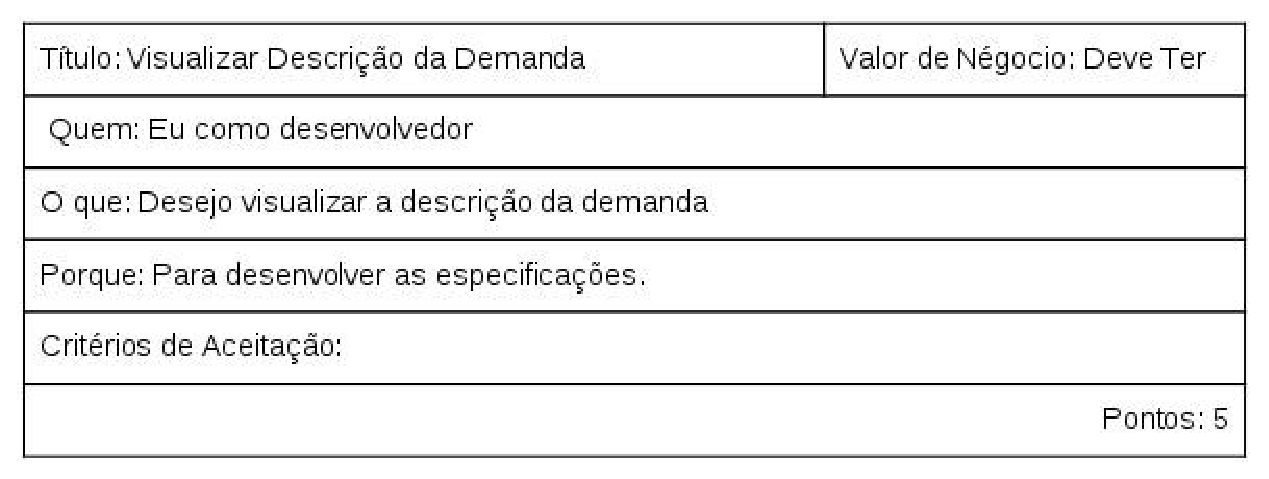
\includegraphics[keepaspectratio=true,scale=0.8]{figuras/iteracao_1/historia_4.eps}
						    \caption{Iteração 1 - História de Usuário}
						    \label{fig:historia1}
						\end{figure}

					\item \textbf{História 05}
						\begin{figure}[H]
						    \centering
							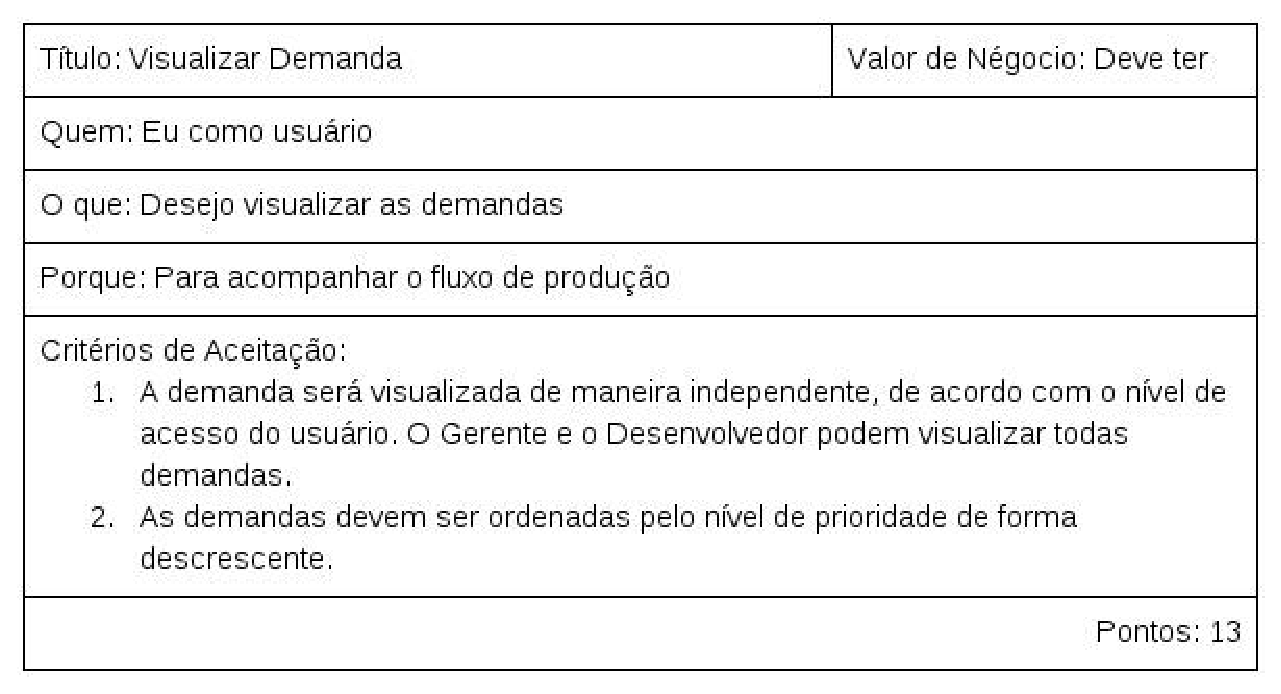
\includegraphics[keepaspectratio=true,scale=0.8]{figuras/iteracao_1/historia_5.eps}
						    \caption{Iteração 1 - História de Usuário}
						    \label{fig:historia1}
						\end{figure}
				\end{enumerate}
		\end{enumerate}

	\item \textbf{Épico:} Gerenciamento de Usuário
		\begin{enumerate}
			\item \textbf{Feature:} Acesso de Usuário
				\begin{enumerate}
					\item \textbf{História 06}
						\begin{figure}[H]
						    \centering
							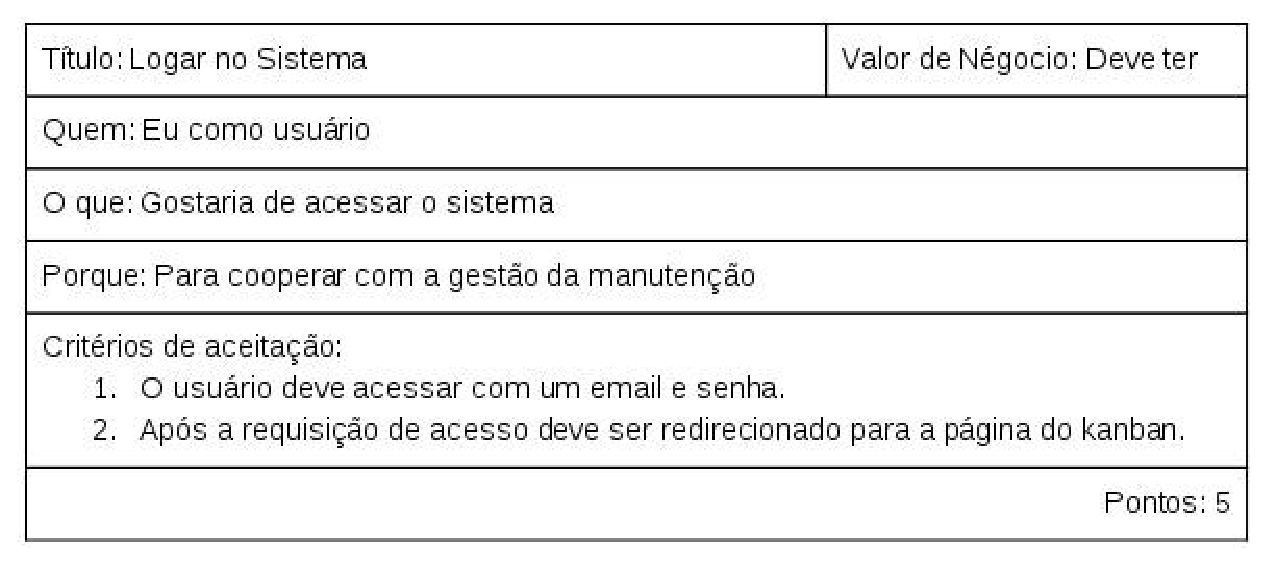
\includegraphics[keepaspectratio=true,scale=0.8]{figuras/iteracao_1/historia_6.eps}
						    \caption{Iteração 1 - História de Usuário}
						    \label{fig:historia1}
						\end{figure}
				\end{enumerate}
		\end{enumerate}
\end{enumerate}